\documentclass[12pt, a4paper]{article}

\usepackage{pdfpages}
\usepackage{biblatex}
\addbibresource{bibliography.bib}
\usepackage{tikz}
\usetikzlibrary{automata, positioning, arrows}

\tikzset{
    ->, 
    >=stealth, 
    node distance=3cm, 
    every state/.style={thick, fill=gray!10}, 
    initial text=$ $
}

\title{Progress Report\\Automata that move both ways}
\author{James Parkinson\\2005821}

\begin{document}
\maketitle

\section{Introduction}

Standard finite automata (such as DFA and NFA) move over the input word in a single direction, hence only reading it once, and these automata are known to only recognise regular languages. This project will study a different class of finite automata called two way finite automata (such as 2DFA and 2NFA) which can move in both directions over the input word, allowing for multiple passes over it. Surprisingly, these two way automata still only recognise regular languages which means there exists conversions between two way automata and one way automata, which will be implemented in code as a starting point for this project.

However, the main goal of this project is to produce software that performs the conjunction of two way deterministic finite transducers (2DFT), which are a type of two way automata that output a string of characters (or the empty string) at each transition that form an output word once the automata terminates. This results in the simulation of a partial function $f:\Sigma^* \rightarrow \Gamma^*$ where $\Sigma$ and $\Gamma$ are the input and output alphabets of the transducer respectively. More specifically, if we have a transducer $A$ that simulates a function $f:\Sigma^* \rightarrow \Gamma^*$ and a transducer $B$ that simulates a function $g:\Gamma^* \rightarrow \Delta^*$, the software would take $A$ and $B$ as input and return a new transducer $C$ that simulates the composition $g \circ f : \Sigma^* \rightarrow \Delta^*$.

\section{Background research}
\subsection{Academic resources}
Many sources have been identified that will be useful for this project, some of the key resources have been listed in the references section of this report, and a brief description of each one will be given here.

\cite{toolbox} is a book called An Automata Toolbox by Mikołaj Bojańczyk and Wojciech Czerwiński, which contains a vast amount of information about automata theory. The part of the book that is most important for this project is chapter 13.3 "Deterministic two-way transducers" which includes a very clear definition of deterministic two-way transducers, as well as a proof that shows 2DFTs are closed under composition which is what this project is trying to reproduce in software.

\cite{chytil} is a paper titled "Serial composition of 2-way finite-state transducers and simple programs on strings" by M. P. Chytil and V. J{\'a}kl that provides another proof for closure under composition for 2DFTs.

\cite{2-1} is a paper titled "The Reduction of Two-Way Automata To One-Way Automata" by J.C. Shepherdson that provides a proof that for every 2DFA there exists an equivalent 1DFA and provides a construction that can be used to create a non-minimal one-way automata given a two-way automata.

\cite{note} is a paper titled "A note on the reduction of two-way automata to one-way automata" by Moshe Y. Vardi that provides an alternate proof for reducing two way automata to one way automata using subset construction, instead of crossing sequence analysis as used in \cite{2-1}

\subsection{Pre-existing software}
During the research phase multiple software solutions for finite state automata were found, however all of them seemed to only focus on one way state machines such as DFA, NFA and PDA. None of the pre-existing software that was found included any implementation of two way automata such as 2DFA, 2NFA and 2DFT, so as this project aims to implement some functionality for two way automata including 2DFA and 2DFT it will be providing functionality that is not currently available.
\pagebreak
\section{Current state of the project}
As shown in section 5 of the project specification, the first 6 weeks of term was spent gathering resources and reading through proofs in order to understand them for when the software implementation begins in week 7. Then from week 7 to 10 the software implementation started, which would continue into term 2.

The project progressed as planned during the first 6 weeks, plenty of resources were gathered and the proofs had been read through multiple times as I tried to fully understand them. Then during the start of week 7 I set up the git repository and started to write the first few lines of code.

However, I fell ill at the end of week 7 and didn't recover fully until the middle of week 9. This greatly affected my ability to work on the project as I was bedridden for the majority of week 8 which also impacted my other responsibilities such as other coursework and society exec obligations. When I recovered enough to start working again I had to first catch up with the backlog of everything I had missed, which delayed me getting back to the project even more than I first expected.

To make up for this lost time, I am going to modify the timetable I gave in the specification by adding on two extra weeks for implementing software and reducing the amount of time spent investigating complexity. The full updated timetable for term 2 will be shown in the next section of the report.

\section{Timetable for Term 2}

As mentioned before, I have updated the timetable for term 2 to add an extra two weeks for software development by reducing the time allocated to investigating the increase in complexity after these functions have been performed.

\begin{center}
    \begin{tabular}{| c | p{8cm} |}
        \hline
        \textbf{Week} & \textbf{Task} \\
        \hline
        \multicolumn{2}{|c|}{\textit{Christmas holiday}}\\
        \hline
        \multicolumn{2}{|c|}{\textbf{Term 2}} \\
        \hline
        W1-W2 & Implement 2DFA to 1DFA \\
        W3-W5 & Implement 2DFT composition \\
        W6-W7 & Investigating Complexity \\
        W8-10 & Project presentation / Final report write up \\
        \hline
        \multicolumn{2}{|c|}{\textit{Easter holiday}}\\
        \hline
        \multicolumn{2}{|c|}{\textbf{Term 3}}\\
        \hline
        W1 & Final report\\
        \hline
    \end{tabular}
\end{center}

No tasks have been assigned during the christmas and easter holidays since I cannot guarantee how much available time I will have, however I will still be working on the project to some degree during these times.

\section{Project Management + Reflection}
During term 1, I allocated parts of my timetable to work solely on the project as I found that having a regular set time every week to work on the project really helped me to stay on track. The project has gone okay so far, although falling ill made me lose a lot of time and pushed back where I wanted to be by the end of this term by a lot, so I am going to make up for that lost time during term 2 and also over the christmas holidays as much as I can.

\pagebreak
\printbibliography


\appendix
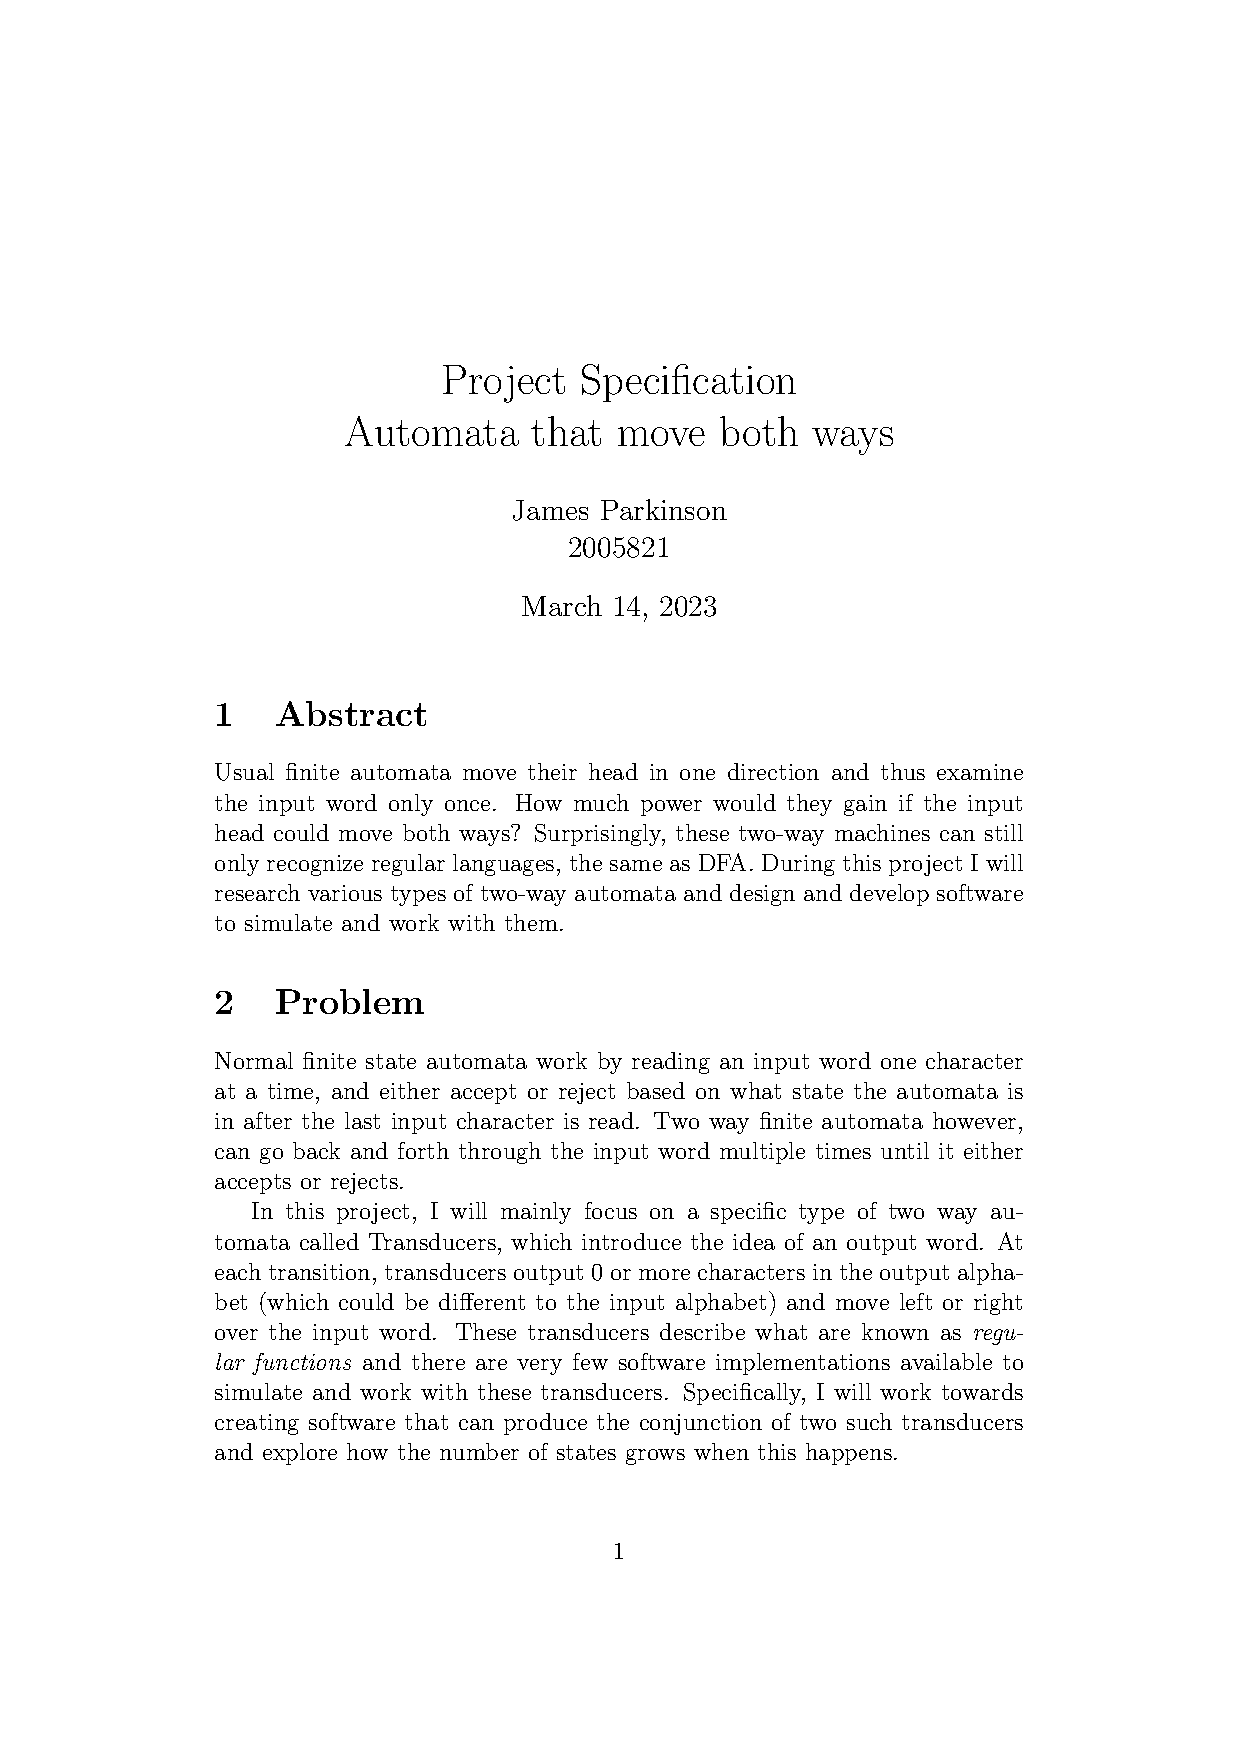
\includepdf[pages=-]{../spec/spec.pdf}

\end{document}